\documentclass[@BEAMER_OPTIONS@]{beamer}
    @USE_PGFPAGES@

    \usetheme{Stockton}
    \setbeamertemplate{navigation symbols}{}
    \setbeamertemplate{note page}[plain]

    \usepackage[utf8]{inputenc}
    \usepackage{graphicx}
    \usepackage{subfigure}
    \usepackage{tikz}
    \usepgflibrary{arrows}
    \usetikzlibrary{decorations.pathreplacing,patterns,shapes}
    \tikzstyle{every picture}=[semithick,>=stealth,remember picture]
    \definecolor{darkblue}{rgb}{0,0,0.5}
    \definecolor{darkred}{rgb}{0.75,0,0.0}
    \usepackage{listings}
    \lstset{
        language=C++,
        basicstyle=\footnotesize\rmfamily,
        numbers=left,
        numberstyle=\tiny,
        aboveskip=-0.02\baselineskip,
        belowskip=-0.02\baselineskip,
        columns=flexible,
        extendedchars=false,
        showstringspaces=false
        }
    \newcommand{\code}[1]{\lstinline|#1|}

    \title{VexCL}
    \subtitle{Vector Expression Template Library for OpenCL}

    \author{Denis Demidov}
    \institute{
        Supercomputer Center of Russian Academy of Sciences\\
        Kazan Federal University
    }
    \date{Meeting C++, 9./10.11.12}

\begin{document}

%----------------------------------------------------------------------------
\begin{frame}{}
    \titlepage
\end{frame}

\note{ }

%----------------------------------------------------------------------------
\begin{frame}{}
    \begin{description}[\;]
        \item[VexCL:] {\color{pacificorange}V}ector {\color{pacificorange}ex}pression
            template library for Open{\color{pacificorange}CL}
            \begin{itemize}
                \item Created for ease of C++ based OpenCL developement.
                \item The source code is publicly available\footnote{
                    \href{https://github.com/ddemidov/vexcl}
                    {https://github.com/ddemidov/vexcl}
                    }
                    under MIT license.
                \item \emph{This is not a C++ bindings library!}
            \end{itemize}
    \end{description}
    \tableofcontents[hideallsubsections]
\end{frame}

\note[itemize]{
\item VexCL is a vector expression template library for OpenCL. It uses
    template metaprogramming techniques (in particular, expression templates)
    to provide an intuitive notation for vector and matrix operations.
\item The source code of the library is available on GitHub. It is distributed
    under MIT license, so you are basically free to do whatever you want with
    the library.
\item I would like to note that this is not another C++ bindings library. VexCL
    is designed to work with standard C++ bindings for OpenCL that are provided
    by the Khronos group.
}

\section{Motivation}

\subsection{Hello OpenCL}

%----------------------------------------------------------------------------
\begin{frame}[fragile]{Hello OpenCL: vector sum}
    \begin{block}{Vector sum}
        \begin{itemize}
            \item $A$, $B$, and $C$ are large vectors.
            \item Compute $C = A + B$.
        \end{itemize}
    \end{block}
    \begin{block}{Overview of OpenCL solution}
        \begin{enumerate}
            \item Initialize OpenCL context on supported device.
            \item Allocate memory on the device.
            \item Transfer input data to device.
            \item Run your computations on the device.
            \item Get the results from the device.
        \end{enumerate}
    \end{block}
\end{frame}

\note[itemize]{
\item Let's start with a motivating example. This is classical hello world
    example for OpenCL: addition of two large vector.
\item To do anything with the OpenCL, you need to perform some standard steps,
    like context initialization, memory allocation and transfer, and the
    computations that you needed to do in the first place.
\item So let's look at how these steps are done with native OpenCL API.
}

%----------------------------------------------------------------------------
\begin{frame}[fragile]{Hello OpenCL: vector sum}
    \begin{exampleblock}{1. Query platforms}
        \begin{lstlisting}
std::vector<cl::Platform> platform;
cl::Platform::get(&platform);

if ( platform.empty() ) {
    std::cerr << "OpenCL platforms not found." << std::endl;
    return 1;
}
        \end{lstlisting}
    \end{exampleblock}
\end{frame}

\note[itemize]{
\item First, we need to enumerate OpenCL platforms. Platform is an OpenCL
    implementation by particular provider. Examples are NVIDIA, AMD or Intel
    platforms.
}

%----------------------------------------------------------------------------
\begin{frame}[fragile]{Hello OpenCL: vector sum}
    \begin{exampleblock}{2. Get first available GPU device}
        \begin{lstlisting}[firstnumber=last]
cl::Context context;
std::vector<cl::Device> device;
for(auto p = platform.begin(); device.empty() && p != platform.end(); p++) {
    std::vector<cl::Device> pldev;
    try {
        p->getDevices(CL_DEVICE_TYPE_GPU, &pldev);
        for(auto d = pldev.begin(); device.empty() && d != pldev.end(); d++) {
            if (!d->getInfo<CL_DEVICE_AVAILABLE>()) continue;
            device.push_back(*d);
            context = cl::Context(device);
        }
    } catch(...) {
        device.clear();
    }
}
if (device.empty()) {
    std::cerr << "GPUs not found." << std::endl;
    return 1;
}
        \end{lstlisting}
    \end{exampleblock}
\end{frame}

\note[itemize]{
\item Once we have the list of platforms, we may pick a compute device that
    suites us. In this example we just get first available device that we are
    able to create an OpenCL context on.
}

%----------------------------------------------------------------------------
\begin{frame}[fragile]{Hello OpenCL: vector sum}
    \begin{exampleblock}{3. Create kernel source}
        \begin{lstlisting}[firstnumber=last]
const char source[] =
    "kernel void add(\n"
    "       uint n,\n"
    "       global const float *a,\n"
    "       global const float *b,\n"
    "       global float *c\n"
    "       )\n"
    "{\n"
    "    uint i = get_global_id(0);\n"
    "    if (i < n) {\n"
    "       c[i] = a[i] + b[i];\n"
    "    }\n"
    "}\n";
        \end{lstlisting}
    \end{exampleblock}
\end{frame}

\note[itemize]{
\item Next thing to do is to compile the compute kernels that we will use.
\item With OpenCL, the kernels are compiled at runtime, because OpenCL supports
    wide range of hardware, and each device may have its own set of
    instructions.
\item Here we create string representation of a kernel source.
}

%----------------------------------------------------------------------------
\begin{frame}[fragile]{Hello OpenCL: vector sum}
    \begin{exampleblock}{4. Compile kernel}
        \begin{lstlisting}[firstnumber=last]
cl::Program program(context, cl::Program::Sources(
            1, std::make_pair(source, strlen(source))
            ));
try {
    program.build(device);
} catch (const cl::Error&) {
    std::cerr
        << "OpenCL compilation error" << std::endl
        << program.getBuildInfo<CL_PROGRAM_BUILD_LOG>(device[0])
        << std::endl;
    return 1;
}
cl::Kernel add_kernel = cl::Kernel(program, "add");
        \end{lstlisting}
    \end{exampleblock}
    \begin{exampleblock}{5. Create command queue}
        \begin{lstlisting}[firstnumber=last]
cl::CommandQueue queue(context, device[0]);
        \end{lstlisting}
    \end{exampleblock}
\end{frame}

\note[itemize]{
\item Then we compile an OpenCL program and create a kernel object.
\item We also create the command queue for OpenCL. All OpenCL operations are
    submitted to a command queue. In general, operations submitted to the same
    queue are performed sequentially.
\item And now we are basically done with initialization. All of the above
    operations are usually done once per program lifetime.
}

%----------------------------------------------------------------------------
\begin{frame}[fragile]{Hello OpenCL: vector sum}
    \begin{exampleblock}{6. Prepare input data, transfer it to device}
        \begin{lstlisting}[firstnumber=last]
const unsigned int N = 1 << 20;
std::vector<float> a(N, 1), b(N, 2), c(N);

cl::Buffer A(context, CL_MEM_READ_ONLY | CL_MEM_COPY_HOST_PTR,
        a.size() * sizeof(float), a.data());

cl::Buffer B(context, CL_MEM_READ_ONLY | CL_MEM_COPY_HOST_PTR,
        b.size() * sizeof(float), b.data());

cl::Buffer C(context, CL_MEM_READ_WRITE,
        c.size() * sizeof(float));
        \end{lstlisting}
    \end{exampleblock}
\end{frame}

\note[itemize]{
\item Next, we need to allocate some device memory and transfer input
    data to the device.
\item The input data is prepared at host in this example. A and B vectors would
    hold ones and twos. This is not very interesting example, but then hello
    world programs never are.
}

%----------------------------------------------------------------------------
\begin{frame}[fragile]{Hello OpenCL: vector sum}
    \begin{exampleblock}{7. Set kernel arguments}
        \begin{lstlisting}[firstnumber=last]
add_kernel.setArg(0, N);
add_kernel.setArg(1, A);
add_kernel.setArg(2, B);
add_kernel.setArg(3, C);
        \end{lstlisting}
    \end{exampleblock}
    \begin{exampleblock}{8. Launch kernel}
        \begin{lstlisting}[firstnumber=last]
queue.enqueueNDRangeKernel(add_kernel, cl::NullRange, N, cl::NullRange);
        \end{lstlisting}
    \end{exampleblock}
    \begin{exampleblock}{9. Get result back to host}
        \begin{lstlisting}[firstnumber=last]
queue.enqueueReadBuffer(C, CL_TRUE, 0, c.size() * sizeof(float), c.data());
std::cout << c[42] << std::endl; // Should get '3' here.
        \end{lstlisting}
    \end{exampleblock}
\end{frame}

\note[itemize]{
\item And now we have everything we need to launch the compute kernel.
\item We set the kernel parameters and submit the kernel to the command queue.
\item Then we transfer the results back to host and see what we got. Here, if
    everything went well, we should get 'three' on standard output.
\item Well, this the ugliest hello world program I ever seen.
\item You will surely agree that a hello world program should fit on one slide.
    And 71 lines of code for a hello world is scary.
\item Well, VexCL tries to soften the blow for its users. And indeed, with
    VexCL I am able to fit this example on a single slide.
}

\subsection{Hello VexCL}

%----------------------------------------------------------------------------
\begin{frame}[fragile]{Hello VexCL: vector sum}
    \begin{exampleblock}{This is much shorter!}
        \begin{lstlisting}
std::cout << 3 << std::endl;
        \end{lstlisting}
    \end{exampleblock}
\end{frame}

\note[itemize]{
\item $\ddot\smile$
}

%----------------------------------------------------------------------------
\begin{frame}[fragile]{Hello VexCL: vector sum}
    \begin{exampleblock}{Get all available GPUs}
        \begin{lstlisting}
vex::Context ctx( vex::Filter::Type(CL_DEVICE_TYPE_GPU) );
if ( !ctx.size() ) {
    std::cerr << "GPUs not found." << std::endl;
    return 1;
}
        \end{lstlisting}
    \end{exampleblock}
    \begin{exampleblock}{Prepare input data, transfer it to device}
        \begin{lstlisting}[firstnumber=last]
std::vector<float> a(N, 1), b(N, 2), c(N);
vex::vector<float> A(ctx.queue(), a);
vex::vector<float> B(ctx.queue(), b);
vex::vector<float> C(ctx.queue(), N);
        \end{lstlisting}
    \end{exampleblock}
    \begin{exampleblock}{Launch kernel, get result back to host}
        \begin{lstlisting}[firstnumber=last]
C = A + B;
vex::copy(C, c);
std::cout << c[42] << std::endl;
        \end{lstlisting}
    \end{exampleblock}
\end{frame}

\note[itemize]{
\item But seriosly, here is the 'Hello VexCL' code.
\item The first line is the context initialization. We provide a device filter
    to the context constructor and get all compute devices that satisfy the
    filter. Here we filter by type and get all available GPUs.
\item Data allocation and transfer is also simplified. \code{vex::vector}
    constructor allocates memory on device and possibly transfers initial data
    as well. The parameters here are list of command queues and either size or
    input host vector.
\item Line ten does what's needs to be done here. This simple expression leads
    to automatic kernel generation and launch. And then we copy the results
    back to host and see what we got.
\item I hope that you agree this code is much simpler and more pleasant to
    write or read.
}

\section{Basic interface}

%----------------------------------------------------------------------------
\begin{frame}[shrink=5]{}
    \tableofcontents[currentsection,hideothersubsections]
\end{frame}

\note[itemize]{
\item Now let's talk about basic VexCL interface. The main parts are context
    initialization, vector arithmetic, such operations as reductions, stencil
    convolutions, sparse matrix -- vector products, and multioperations.
}

\subsection{Device selection}

%----------------------------------------------------------------------------
\begin{frame}[fragile]{Device selection}
    \begin{itemize}
        \item Multi-device and multi-platform computations are supported.
        \item VexCL context is initialized from combination of device filters.
        \item Device filter is a boolean functor acting on \code{const
            cl::Device&}.
    \end{itemize}
    \vspace{-0.5\baselineskip}
    \begin{overlayarea}{\textwidth}{0.4\textheight}
    \begin{exampleblock}{Initialize VexCL context on selected devices}
        \begin{onlyenv}<1>
        \begin{lstlisting}
vex::Context ctx( vex::Filter::All );
        \end{lstlisting}
        \end{onlyenv}
        \begin{onlyenv}<2|handout:0>
        \begin{lstlisting}
vex::Context ctx( vex::Filter::Type(CL_DEVICE_TYPE_GPU) );
        \end{lstlisting}
        \end{onlyenv}
        \begin{onlyenv}<3|handout:0>
        \begin{lstlisting}
vex::Context ctx(
    vex::Filter::Type(CL_DEVICE_TYPE_GPU) &&
    vex::Filter::Platform("AMD")
    );
        \end{lstlisting}
        \end{onlyenv}
        \begin{onlyenv}<4|handout:0>
        \begin{lstlisting}
vex::Context ctx(
    vex::Filter::Type(CL_DEVICE_TYPE_GPU) &&
    [](const cl::Device &d) {
        return d.getInfo<CL_DEVICE_GLOBAL_MEM_SIZE>() >= 4_GB;
    });
        \end{lstlisting}
        \end{onlyenv}
    \end{exampleblock}
    \end{overlayarea}
    \begin{figure}
        \uncover<1-2,4>{
            \includegraphics[width=0.25\textwidth]{tesla.png}\quad
        }
        \uncover<1-3>{
            \includegraphics[width=0.25\textwidth]{radeon.png}\quad
        }
        \uncover<1>{
            \includegraphics[width=0.2\textwidth]{intel.png}
        }
    \end{figure}
\end{frame}

\note[itemize]{
\item VexCL can transparently work with several compute devices that are
    present on your system.
\item We initialize the VexCL context with a device filter. The device filter
    is a simple functor that acts on cl::Device reference and returns a boolean
    value. Several standard filters are provided and you can write your own
    filters.
\item Let's assume that we have an NVIDIA GPU, an AMD GPU, and an Intel CPU
    installed.
    \begin{enumerate}
        \item The standard 'All' Filter select any device available, so we end
            with three devices in our context.
        \item If we want to select only GPUs, then we can filter the devices by
            type.
        \item It is also possible to combine the device filters with logical
            operators.  Here we select a GPU that is provided by AMD OpenCL
            platform.
        \item And here is an example of a custom filter. Here it selects any
            device that has at least 4GB of memory.
    \end{enumerate}
}

%----------------------------------------------------------------------------
\begin{frame}[fragile]{Exclusive device access}
    \begin{itemize}
        \item \code{vex::Filter::Exclusive()} wraps normal filters to allow
            exclusive access to devices.
        \item Useful for cluster environments.
        \item An alternative to NVIDIA's exclusive compute mode for other
            vendors hardware.
        \item Based on Boost.Interprocess file locks in temp directory.
    \end{itemize}
    \begin{exampleblock}{}
        \begin{lstlisting}
vex::Context ctx( vex::Filter::Exclusive (
    vex::Filter::DoublePrecision &&
    vex::Filter::Env
    ) );
        \end{lstlisting}
    \end{exampleblock}
\end{frame}

\note[itemize]{
\item Often we want to get an exclusive access to our compute devices. This is
    especially true in a clustered environments, where job manager may tell you
    how many devices are available, but it usually doesn't know which exactly.
\item The Exclusive filter wrapper lets you do this. Internally, lock
    files are created for each compute device present in the system.
\item This obviously will only work between VexCL programs that explicitly ask
    for an exclusive access.
}

%----------------------------------------------------------------------------
\begin{frame}[fragile]{What if OpenCL context is initialized elsewhere?}
    \begin{itemize}
        \item You don't \emph{have to} initialize \code{vex::Context}.
        \item \code{vex::Context} is just a convenient container that holds
            OpenCL contexts and queues.
        \item \code{vex::Context::queue()} returns
            \code{std::vector<cl::CommandQueue>}.\\ This may come from
            \emph{elsewhere}.
    \end{itemize}
    \begin{exampleblock}{}
        \begin{lstlisting}
std::vector<cl::CommandQueue> my_own_vector_of_opencl_command_queues;
// ...
vex::vector<double> x(my_own_vector_of_opencl_command_queues, n);
        \end{lstlisting}
    \end{exampleblock}
    \begin{itemize}
        \item Each queue should correspond to a separate device.
        \item Different VexCL objects may be initialized with different queue
            lists.
        \item Operations are submitted to the queues of the vector that is
            being assigned to.
    \end{itemize}
\end{frame}

\note[itemize]{
\item So, what if you already have some OpenCL project and you do your own
    initialization that you are happy with?
\item VexCL may be used in this case as well, because VexCL Context is just a
    convenice class that holds OpenCL contexts and queues. Every (or almost
    every) VexCL object recieves a queue list at initialization. And this list
    may come from VexCL context or from your own initialization routine.
\item The only assumption that VexCL makes about the list is that each queue in
    it belongs to a different device.
\item It is even possible to initialize different objects with different queue
    lists.  You may want to do this to manually partition the load between
    devices, or to create some non-linear flow in your program.
}

\subsection{Vector arithmetic}

%----------------------------------------------------------------------------
\begin{frame}[fragile]{Vector allocation and arithmetic}
    \begin{exampleblock}{Hello VexCL example}
        \begin{onlyenv}<1|handout:0>
        \begin{lstlisting}[escapechar=!]
vex::Context ctx( !\color{darkred}{vex::Filter::Name("Tesla")}! );
        \end{lstlisting}
        \end{onlyenv}
        \begin{onlyenv}<2|handout:0>
        \begin{lstlisting}[escapechar=!]
vex::Context ctx( !\color{darkred}{vex::Filter::Type(CL\_DEVICE\_TYPE\_GPU)}! );
        \end{lstlisting}
        \end{onlyenv}
        \begin{onlyenv}<3>
        \begin{lstlisting}[escapechar=!]
vex::Context ctx( !\color{darkred}{vex::Filter::DoublePrecision}! );
        \end{lstlisting}
        \end{onlyenv}
        \begin{lstlisting}[firstnumber=last]

vex::vector<float> A(ctx.queue(), N); A = 1;
vex::vector<float> B(ctx.queue(), N); B = 2;
vex::vector<float> C(ctx.queue(), N);

C = A + B;
        \end{lstlisting}
    \end{exampleblock}
    \begin{figure}
        \begin{tikzpicture}
            \draw (0,3.0) rectangle +(8,0.1);
            \draw (0,3.0) grid[step=0.1] +(8,0.1);
            \draw (-0.3,3.1) node{A};

            \draw (0,2.5) rectangle +(8,0.1);
            \draw (0,2.5) grid[step=0.1] +(8,0.1);
            \draw (-0.3,2.6) node{B};

            \draw (0,2.0) rectangle +(8,0.1);
            \draw (0,2.0) grid[step=0.1] +(8,0.1);
            \draw (-0.3,2.1) node[anchor=center]{C};

            \uncover<1-3> {
            \draw (1,0.5) node{\includegraphics[width=0.2\textwidth]{tesla.png}};
            }

            \uncover<2-3> {
            \draw (4,0.5) node{\includegraphics[width=0.2\textwidth]{radeon.png}};
            }

            \uncover<3> {
            \draw (7.5,0.5) node{\includegraphics[width=0.16\textwidth]{intel.png}};
            }

            \uncover<1|handout:0> {
            \draw[->,darkred,style=dashed] (0,3.2) -- (0,1.8)
                .. controls +(east:0.5) and +(north west:0.5) ..
                (1.4,1.5);
            \draw[->,darkred,style=dashed] (8,3.2) -- (8,1.8)
                .. controls +(west:0.5) and +(north east:0.5) ..
                (1.6,1.5);
            }

            \uncover<2|handout:0> {
            \draw[->,darkred,style=dashed] (0,3.2) -- (0,1.8)
                .. controls +(east:0.5) and +(north west:0.5) ..
                (1.4,1.5);
            \draw[->,darkred,style=dashed] (4,3.2) -- (4,1.8)
                .. controls +(west:0.5) and +(north east:0.5) ..
                (1.6,1.5);

            \draw[->,darkred,style=dashed] (4,3.2) -- (4,1.8)
                .. controls +(east:0.1) and +(north west:0.2) ..
                (4.4,1.5);
            \draw[->,darkred,style=dashed] (8,3.2) -- (8,1.8)
                .. controls +(west:0.5) and +(north east:0.5) ..
                (4.6,1.5);
            }

            \uncover<3> {
            \draw[->,darkred,style=dashed] (0,3.2) -- (0,1.8)
                .. controls +(east:0.5) and +(north west:0.5) ..
                (1.4,1.5);
            \draw[->,darkred,style=dashed] (3.5,3.2) -- (3.5,1.8)
                .. controls +(west:0.5) and +(north east:0.5) ..
                (1.6,1.5);

            \draw[->,darkred,style=dashed] (3.5,3.2) -- (3.5,1.8)
                .. controls +(east:0.5) and +(north west:0.2) ..
                (4.4,1.5);
            \draw[->,darkred,style=dashed] (7,3.2) -- (7,1.8)
                .. controls +(west:0.5) and +(north east:0.5) ..
                (4.6,1.5);

            \draw[->,darkred,style=dashed] (7,3.2) -- (7,1.8) -- (7.4,1.5);
            \draw[->,darkred,style=dashed] (8,3.2) -- (8,1.8) -- (7.6,1.5);
            }
        \end{tikzpicture}
    \end{figure}
\end{frame}

\note[itemize]{
\item Now that we know how to initialize VexCL context, let's see how device
    vectors are allocated.
\item Here we allocate three vectors, and initialize two of them with
    constant values.
\item Each vector receives a list of queues at initialization.  Since each
    queue corresponds to a specific device, vectors know where to put their
    data to.
    \begin{enumerate}
        \item For example, if we only have the Tesla card in our context, then
            it will hold the complete memory for all of our vectors.
        \item If we use both of the available GPUs, then the vectors will be
            split between the devices. This split is by default proportional to
            the GPU bandwidth and is guaranteed to be consistent for vectors of
            the same size. This consistency allows VexCL to run computations
            independently on all devices in context.
        \item If we add the CPU to the context, it will get smaller share of
            the data and arithmetic operations.
    \end{enumerate}
\item Care must be taken with the use of several devices. VexCL tries to split
    the memory as fair as it can, but it is probable that your program will
    run at the speed of the slowest device.
}

%----------------------------------------------------------------------------
\begin{frame}[fragile]{What may be used in vector expressions?}
    \begin{itemize}
        \item All vectors in expression have to be \emph{compatible}:
            \begin{itemize}
                \item Have same size
                \item Located on same devices
            \end{itemize}
        \item What may be used:
            \begin{itemize}
                \item Scalar values
                \item Arithmetic, bitwise, logical operators
                \item Builtin OpenCL functions
                \item User-defined functions
            \end{itemize}
    \end{itemize}
    \begin{exampleblock}{}
        \begin{lstlisting}
std::vector<float> x(n);
std::generate(x.begin(), x.end(), rand);

vex::vector<float> X(ctx.queue(), x);
vex::vector<float> Y(ctx.queue(), n);
vex::vector<float> Z(ctx.queue(), n);

Y = 42;
Z = sqrt(2 * X) + pow(cos(Y), 2.0);
        \end{lstlisting}
    \end{exampleblock}
\end{frame}

\note[itemize]{
\item So, what kind of expressions can you use in VexCL?
\item First, any vectors used in an expression have to be compatible.
\item If this requirement is satisfied, then expressions may combine
    vectors and scalars with almost any binary operators. OpenCL math functions
    and user-defined functions are also available.
}

\subsection{Reductions}

%----------------------------------------------------------------------------
\begin{frame}[fragile]{Reductions}
    \begin{itemize}
        \item Class \code{vex::Reductor<T, kind>} allows to reduce arbitrary
            \emph{vector expression} to a single value of type \code{T}.
        \item Supported reduction kinds: \code{SUM}, \code{MIN}, \code{MAX}
    \end{itemize}
    \begin{exampleblock}{Inner product}
        \begin{lstlisting}
vex::Reductor<double, vex::SUM> sum(ctx.queue());
double s = sum(x * y);
        \end{lstlisting}
    \end{exampleblock}
    \begin{exampleblock}{Number of elements in x between 0 and 1}
        \begin{lstlisting}
vex::Reductor<size_t, vex::SUM> sum(ctx.queue());
size_t n = sum( (x > 0) && (x < 1) );
        \end{lstlisting}
    \end{exampleblock}
    \begin{exampleblock}{Maximum distance from origin}
        \begin{lstlisting}
vex::Reductor<double, vex::MAX> max(ctx.queue());
double d = max( sqrt(x * x + y * y) );
        \end{lstlisting}
    \end{exampleblock}
\end{frame}

\note[itemize]{
\item Reduction is an operation of reducing a vector to a single value.
\item The most frequent types are summation and finding minimum or maximum
    element of a vector.
\item VexCL provides Reductor functor that accepts any valid vector expression
    as a parameter.
\item For example, to compute an inner product of two vectors we compute sum of
    their elementwise product.
\item To find number of elements in vector x that are greater than zero and
    less than one, we compute sum of the corresponding boolean expression.
\item And to find the maximum distance from axis origin for a set of
    two-dimensional points, we compute exactly that: max of their radius.
}

\subsection{User-defined functions}

%----------------------------------------------------------------------------
\begin{frame}[fragile]{User-defined functions}
    \begin{itemize}
        \item Users may define functions to be used in vector expressions:
            \begin{itemize}
                \item Provide function body
                \item Define return type and argument types
            \end{itemize}
    \end{itemize}
    \begin{exampleblock}{Defining a function}
        \begin{lstlisting}[escapechar=!]
extern const char between_body[] = "return prm1 <= prm2 && prm2 <= prm3;";
UserFunction<between_body, bool(double, double, double)> !\color{darkred}{between}!;
        \end{lstlisting}
    \end{exampleblock}
    \begin{exampleblock}{Using a function: number of 2D points in first quadrant}
        \begin{lstlisting}[escapechar=!]
size_t points_in_1q( const vex::Reductor<size_t, vex::SUM> &sum,
    const vex::vector<double> &x, const vex::vector<double> &y )
{
    return sum( !\color{darkred}{between}!(0.0, atan2(y, x), M_PI/2) );
}
        \end{lstlisting}
    \end{exampleblock}
\end{frame}

\note[itemize]{
\item It is possible to define an OpenCL function that may be used with vector
    expressions. You need to provide function body, parameter types, and return
    type.
\item Function body has to be of \code{extern const char} type, to allow its
    use as a template parameter. And it has to be defined at global scope.
\item Inside the body function parameters are always named prm1, prm2, etc.
\item Here we define 'between' function that returns true if its second
    parameter is between its first and third parameters. The UserFunction
    object is stateless, so it may be good idea to define it at global scope
    as well, next to its body.
\item Now we may use the function in expressions. Any vector expression may be
    used as a parameter for a user-defined (or builtin) function.
}

\subsection{Sparse matrix~-- vector products}

%----------------------------------------------------------------------------
\begin{frame}[fragile]{Sparse matrix~-- vector products}
    \begin{itemize}
        \item Class \code{vex::SpMat<T>} holds representation of a sparse
            matrix on compute devices.
        \item Constructor accepts matrix in common CRS format (row indices,
            columns and values of nonzero entries).
        \item SpMV may only be used in additive expressions.
    \end{itemize}
    \begin{exampleblock}{Construct matrix}
        \begin{lstlisting}
vex::SpMat<double> A(ctx.queue(), n, n, row.data(), col.data(), val.data());
        \end{lstlisting}
    \end{exampleblock}

    \begin{exampleblock}{Compute residual value}
        \begin{lstlisting}[firstnumber=last]
// vex::vector<double> u, f, r;
r = f - A * u;
double res = max( fabs(r) );
        \end{lstlisting}
    \end{exampleblock}
\end{frame}

\note[itemize]{
\item Sparse matrix -- vector operation is also provided. A matrix is imported
    from commonly used compressed row storage format.
\item Note that matrix-vector product is not a first-class citizen in vector
    expressions. It uses neighbor values; and neighbors may reside on a
    different compute device. So extra work is needed to exchange data between
    devices. That is why matrix-vector products may only be used in additive
    expressions.
}

\subsection{Stencil convolutions}

%----------------------------------------------------------------------------
\begin{frame}[fragile]{Simple stencil convolutions}
    \begin{figure}
        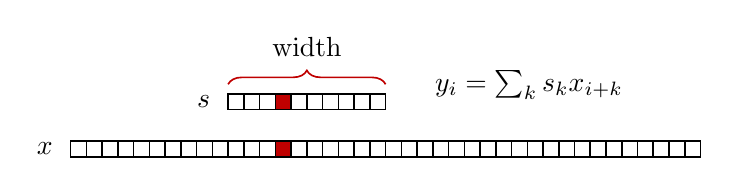
\begin{tikzpicture}
            \draw[fill,darkred] (2.6,0.6) rectangle +(0.2,0.2);
            \draw[fill,darkred] (2.6,0.0) rectangle +(0.2,0.2);

            \draw (0,0) rectangle +(8,0.2);
            \draw (0,0) grid[step=0.2] +(8,0.2);

            \draw (2,0.6) rectangle +(2,0.2);
            \draw (2,0.6) grid[step=0.2] +(2,0.2);

            \draw[darkred,decorate,decoration={brace,amplitude=5},yshift=2]
                (2,0.85) -- (4.,0.85);
            \draw (3,1.4) node{width};

            \draw (1.9,0.7) node[anchor=east]{$s$};
            \draw (-0.1,0.1) node[anchor=east]{$x$};
            \draw (4.5,0.6) node[anchor=south west]{$y_i=\sum_k s_k x_{i+k}$};
        \end{tikzpicture}
    \end{figure}
    \begin{itemize}
        \item Simple stencil is based on a 1D array, and may be used for:
            \begin{itemize}
                \item Signal filters (e.g. averaging)
                \item Differential operators with constant coefficients
                \item \ldots
            \end{itemize}
    \end{itemize}
    \begin{exampleblock}{Moving average with 5-points window}
        \begin{lstlisting}
std::vector<double> sdata(5, 0.2);
vex::stencil<double> s(ctx.queue(), sdata, 2 /* center */);

y = x * s;
        \end{lstlisting}
    \end{exampleblock}
\end{frame}

\note[itemize]{
\item Another commonly used operation is stencil convolution. It may be used to
    filter a one-dimensional signal or to represent a differential operator.
\item A stencil is defined by providing data for its coefficients and
    specifying its center point.
\item To convolve a vector with a stencil you use this simple notation.
\item Stencil convolutions, as well as matrix products, need data from neighbor
    devices; so they may be used only in additive expressions.
}

%----------------------------------------------------------------------------
\begin{frame}[fragile]{User-defined stencil operators}
    \begin{itemize}
        \item Define efficient arbitrary stencil operators:
            \begin{itemize}
                \item Return type
                \item Stencil dimensions (width and center)
                \item Function body
            \end{itemize}
    \end{itemize}
    \begin{block}{Example: nonlinear operator}
        \begin{equation*}
            y_i = x_i + \left( x_{i-1} + x_{i+1} \right)^3
        \end{equation*}
    \end{block}
    \begin{exampleblock}{Implementation}
        \begin{lstlisting}
extern const char custom_op_body[] =
    "double t = X[-1] + X[1];\n"
    "return X[0] + t * t * t;"

vex::StencilOperator<double, 3 /*width*/, 1 /*center*/, custom_op_body>
    custom_op(ctx.queue());

y = custom_op(x);
        \end{lstlisting}
    \end{exampleblock}
\end{frame}

\note[itemize]{
\item It is also possible to define a custom stencil operation. This may be
    used, for example, if the stencil operator is nonlinear.
\item For this you specify return type, width of the stencil, its center, and
    function body.
\item In the function body you access values through X array. Its elements are
    indexed relatively to the stencil center.
}

\subsection{Multivectors \& multiexpressions}

%----------------------------------------------------------------------------
\begin{frame}[fragile]{Multivectors}
    \begin{itemize}
        \item \code{vex::multivector<T,N>} holds \code{N} instances of equally
            sized \code{vex::vector<T>}
        \item Supports all operations that are defined for
            \code{vex::vector<>}.
        \item Transparently dispatches the operations to the underlying
            components.
        \item \code{vex::multivector::operator(uint k)} returns \code{k}-th
            component.
    \end{itemize}
    \begin{exampleblock}{}
        \begin{lstlisting}
vex::multivector<double, 2> X( ctx.queue(), N), Y( ctx.queue(), N);
vex::Reductor<double, vex::SUM> sum(ctx.queue());
vex::SpMat<double> A( ctx.queue(), ... );
std::array<double, 2> v;

// ...

X = sin(v * Y + 1);             // X(k) = sin(v[k] * Y(k) + 1);
v = sum( between(0, X, Y) );    // v[k] = sum( between( 0, X(k), Y(k) ) );
X = A * Y;                      // X(k) = A * Y(k);
        \end{lstlisting}
    \end{exampleblock}
\end{frame}

\note[itemize]{
\item This is in principle all of the basic VexCL operations.
\item What is left are multivectors and multiexpressions.
}

%----------------------------------------------------------------------------
\begin{frame}[fragile]{Multiexpressions}
    \begin{itemize}
        \item Sometimes an operation cannot be expressed with simple
            multivector arithmetics.
    \end{itemize}
    \begin{block}{Example: rotate 2D vector by an angle}
        \vspace{-1\baselineskip}
        \begin{align*}
            y_0 &= x_0 \cos \alpha - x_1 \sin \alpha, \\
            y_1 &= x_0 \sin \alpha + x_1 \cos \alpha.
        \end{align*}
    \end{block}

    \begin{itemize}
        \item Multiexpression is a tuple of normal vector expressions
        \item Its assignment to a multivector is functionally equivalent to
            componentwise assignment, but results in a single kernel launch.
    \end{itemize}
\end{frame}

\note[itemize]{
\item Sometimes it's not possible to express the required operation with simple
    multivector arithmetics.
\item For example, take two-dimensional point rotation operation, which is
    defined as this couple of expressions. X and Y coordinates are mixed
    here, so we either have to split the operation in two, or use a
    multiexpression.
}

%----------------------------------------------------------------------------
\begin{frame}[fragile]{Multiexpressions}
    \begin{itemize}
        \item Multiexpressions may be used with multivectors:
    \end{itemize}
    \begin{exampleblock}{}
        \begin{lstlisting}
// double alpha;
// vex::multivector<double,2> X, Y;

Y = std::tie(
            X(0) * cos(alpha) - X(1) * sin(alpha),
            X(0) * sin(alpha) + X(1) * cos(alpha)  );
        \end{lstlisting}
    \end{exampleblock}
    \begin{itemize}
        \item and with tied vectors:
    \end{itemize}
    \begin{exampleblock}{}
        \begin{lstlisting}
// vex::vector<double> alpha;
// vex::vector<double> odlX, oldY, newX, newY;

vex::tie(newX, newY) = std::tie(
            oldX * cos(alpha) - oldY * sin(alpha),
            odlX * sin(alpha) + oldY * cos(alpha)  );
        \end{lstlisting}
    \end{exampleblock}
    \begin{itemize}
        \item Any expression that is assignable to a vector is valid in a
            multiexpression.
    \end{itemize}
\end{frame}

\note[itemize]{
\item You can assign a tuple of expressions to a multivector, or to a tuple of
    single vectors.
\item In either case, this will result in single kernel launch that will update
    all parts of the result at once.
\item Also note that in the second example we rotate every point by its own
    angle stored in alpha vector.
}

%----------------------------------------------------------------------------
\begin{frame}[fragile]{Copies between host and device memory}
    \begin{exampleblock}{}
        \begin{lstlisting}
vex::vector<double> X;
std::vector<double> x;
double c_array[100];
        \end{lstlisting}
    \end{exampleblock}
    \begin{exampleblock}{Simple copies}
        \begin{lstlisting}
vex::copy(X, x); // From device to host.
vex::copy(x, X); // From host to device.
        \end{lstlisting}
    \end{exampleblock}
    \begin{exampleblock}{STL-like range copies}
        \begin{lstlisting}
vex::copy(X.begin(), X.end(), x.begin());
vex::copy(X.begin(), X.begin() + 100, x.begin());
vex::copy(c_array, c_array + 100, X.begin());
        \end{lstlisting}
    \end{exampleblock}
    \begin{exampleblock}{Inspect or set single element (\emph{slow})}
        \begin{lstlisting}
vex::copy(X, x);
assert(x[42] == X[42]);
X[0] = 0;
        \end{lstlisting}
    \end{exampleblock}
\end{frame}

\note[itemize]{
\item Copies between host and device memory may be done with simple copy
    function that copy the complete vector either way,
\item or, if you need to do partial copy, you can use STL-like syntax.
\item Vectors also overload array subscript operator, so you can have direct
    read or write access to any element of a vector. But this should be used
    with caution because it is slow. The intended use for this is a single
    element access or debugging.
\item Data may also be accessed through iterators, so it is possible to use,
    for example, an STL algorithm with device vector as a temporary solution.
}


\section{Kernel builder}

%----------------------------------------------------------------------------
\begin{frame}{}
    \tableofcontents[currentsection,hideallsubsections]
\end{frame}

\note[itemize]{
\item VexCL has other nice feature, called kernel builder or kernel generator.
    This feature is so nice that it requires a motivating example as an
    introduction, so here it goes.
}

\subsection{Kernel builder}

%----------------------------------------------------------------------------
\begin{frame}[fragile]{Converting generic C++ algorithms to OpenCL
    kernels$^*$}{$^*$Restrictions applied}
    \begin{columns}
        \begin{column}{0.6\textwidth}
            \begin{block}{Motivating example}
                \begin{itemize}
                    \item Let's solve an ODE!
                    \item Let's do it with Boost.odeint!
                        \vspace{\baselineskip}
                    \item Lorenz attractor system:
                \end{itemize}
                \vspace{-1\baselineskip}
                \begin{align*}
                    \dot{x} &= -\sigma \left( x - y \right), \\
                    \dot{y} &= R x - y - xz, \\
                    \dot{z} &= -bz + xy.
                    \label{eq:lorenz}
                \end{align*}
                \begin{itemize}
                    \item We want to solve large number of Lorenz systems, each
                        for a different value of $R$.
                \end{itemize}
            \end{block}
        \end{column}
        \begin{column}{0.4\textwidth}
            \begin{figure}
                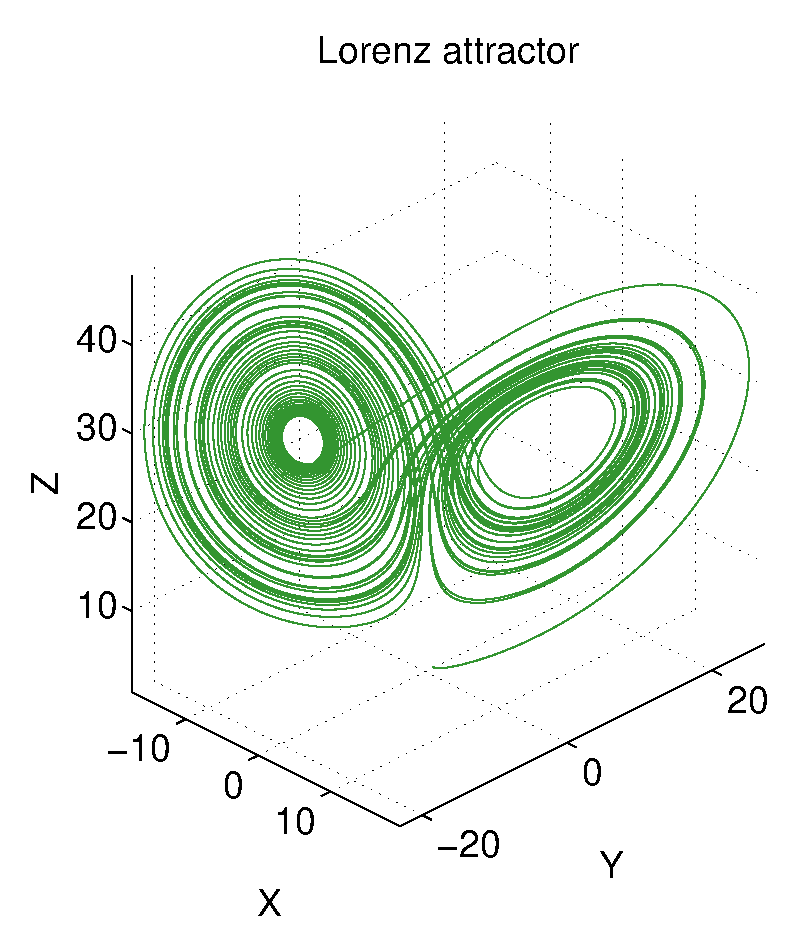
\includegraphics[width=\textwidth]{lorenz}
            \end{figure}
        \end{column}
    \end{columns}
\end{frame}

\note[itemize]{
\item Let us do something interesting now. Namely, lets solve a Lorenz
    attractor system of ordinary differential equations. And let us use
    odeint library that was presented yesterday by Karsten here.
\item Lorenz attractor is a particle that moves according to these governing
    equations. The plot on the right shows an example of particle trajectory in
    time.
\item Since we have to justify the use of an expensive GPU somehow, let us
    solve huge number of these Lorenz systems at once.
\item Each of the systems will have its own value for parameter R. That's why
    this is called a parameter study.
}

%----------------------------------------------------------------------------
\begin{frame}[fragile]{odeint setup}
    \begin{exampleblock}{1. System functor}
        \begin{lstlisting}
typedef vex::vector<double>         vector_type;
typedef vex::multivector<double, 3> state_type;

struct lorenz_system {
    const vector_type &R;
    lorenz_system(const vector_type &R ) : R(R) { }

    void operator()(const state_type &x, state_type &dxdt, double t) {
        dxdt = std::tie(
                    sigma * ( x(1) - x(0) ),
                    R * x(0) - x(1) - x(0) * x(2),
                    x(0) * x(1) - b * x(2)
                );
    }
};
        \end{lstlisting}
    \end{exampleblock}
\end{frame}

\note[itemize]{
\item We will hold current state of the system (or set of attractor
    coordinates) in a multivector with 3 components.
\item To use the odeint library, we have to provide a functor that computes
    right hand side of our equations.
\item The functor has to accept current state, reference to time derivative,
    and current time value. It has to compute the time derivative from current
    state and possibly time.
\item So we accept multivector x here and modify multivector dxdt. Use of VexCL
    multiexpression makes this very simple and effective.
}

%----------------------------------------------------------------------------
\begin{frame}[fragile]{odeint setup}
    \begin{exampleblock}{2. Integration}
        \begin{lstlisting}
state_type  X( ctx.queue(), n );
vector_type R( ctx.queue(), r );

// ... initialize X and R here ...

odeint::runge_kutta4<
        state_type, double, state_type, double,
        odeint::vector_space_algebra, odeint::default_operations
        > stepper;

odeint::integrate_const(stepper, lorenz_system(R), X, 0.0, t_max, dt);
        \end{lstlisting}
    \end{exampleblock}
    \begin{itemize}
        \item That was easy! \uncover<2->{And fast!} \uncover<3->{\alert{But,}}
            \begin{itemize}
                \item<4|alert@4> Runge-Kutta method uses 4 temporary state variables
                    (here stored on GPU).
                \item<4|alert@4> Single Runge-Kutta step results in several
                    kernel launches.
            \end{itemize}
    \end{itemize}
\end{frame}

\note[itemize]{
\item Once we defined our state type and the system functor, we need to create
    the stepper object and run the integration routine. Here we use classic 4th
    order Runge-Kutta method.
\item And that's it! This was really easy. And it was ten times faster than a
    multithreaded CPU variant.
\item But, it could be better.
}

%----------------------------------------------------------------------------
\begin{frame}[fragile,shrink=40]{What if we did this manually?}
    \begin{columns}
        \begin{column}{0.45\textwidth}
            \begin{LARGE}
                \begin{enumerate}
                    \item Create single monolithic kernel that does one step of
                        Runge-Kutta method.
                    \item Launch the kernel in a loop.
                        \vspace{2\baselineskip}
                    \item This is $\approx 10$ times faster!
                        \uncover<2->{\alert{But,}}
                    \item<3|alert@3> We lost the generality odeint offers!
                \end{enumerate}
            \end{LARGE}
        \end{column} \quad \quad
        \begin{column}{0.5\textwidth}
            \begin{exampleblock}{}
                \begin{lstlisting}
double3 lorenz_system(double r, double sigma, double b, double3 s) {
    return (double3)(
        sigma * (s.y - s.x),
        r * s.x - s.y - s.x * s.z,
        s.x * s.y - b * s.z
        );
}

kernel void lorenz_ensemble(
    ulong  n, double sigma, double b,
    const global double *R,
    global double *X,
    global double *Y,
    global double *Z
    )
{
    double r;
    double3 s, dsdt, k1, k2, k3, k4;

    for(size_t gid = get_global_id(0); gid < n; gid += get_global_size(0)) {
        r = R[gid];
        s = (double3)(X[gid], Y[gid], Z[gid]);

        k1 = dt * lorenz_system(r, sigma, b, s);
        k2 = dt * lorenz_system(r, sigma, b, s + 0.5 * k1);
        k3 = dt * lorenz_system(r, sigma, b, s + 0.5 * k2);
        k4 = dt * lorenz_system(r, sigma, b, s + k3);

        s += (k1 + 2 * k2 + 2 * k3 + k4) / 6;

        X[gid] = s.x; Y[gid] = s.y; Z[gid] = s.z;
    }
}
                \end{lstlisting}
            \end{exampleblock}
        \end{column}
    \end{columns}
\end{frame}

\note[itemize]{
\item So, what if we did this manually?
\item We would create a single kernel that would do complete Runge-Kutta
    integration step. By the way, here is the kernel that does just that. It's
    very nice-looking kernel in fact.
\item If we run this kernel in a loop, it would give us our solution. And it
    would be ten times faster than our previous variant. So a hundred times
    faster than a CPU! That's an acceleration!
\item But, odeint has 20 different steppers. We don't want to reimplement all
    of those. Let Karsten here do the job, right?
}

%----------------------------------------------------------------------------
\begin{frame}[fragile]{Convert generic C++ algorithms to OpenCL kernels}
    \begin{enumerate}
        \item Capture the sequence of arithmetic expressions of an algorithm.
        \item Construct OpenCL kernel from the captured sequence.
        \item ???
        \item Use the kernel!
    \end{enumerate}
\end{frame}

\note[itemize]{
\item So, what do we do?
\item The idea is very simple:
    \begin{itemize}
        \item An algorithm (any algorithm) is just a sequence of arithmetic
            expressions.
        \item Let's record the sequence of expressions that, for example,
            Runge-Kutta method does, and let's build an OpenCL kernel from this
            sequence.
    \end{itemize}
}

%----------------------------------------------------------------------------
\begin{frame}[fragile]{Convert generic C++ algorithms to OpenCL kernels}
    \begin{exampleblock}{1. Declare functor operating on
        \code{vex::generator::symbolic<>} values}
        \begin{lstlisting}
typedef vex::generator::symbolic< double > sym_vector;
typedef std::array<sym_vector, 3> sym_state;

struct lorenz_system {
    const sym_vector &R;
    lorenz_system(const sym_vector &R) : R(R) {}
    void operator()(const sym_state &x, sym_state &dxdt, double t) const {
        dxdt[0] = sigma * (x[1] - x[0]);
        dxdt[1] = R * x[0] - x[1] - x[0] * x[2];
        dxdt[2] = x[0] * x[1] - b * x[2];
    }
};
        \end{lstlisting}
    \end{exampleblock}
\end{frame}

\note[itemize]{
\item To capture the expression sequence VexCL provides special symbolic class.
    The class overloads arithmetic operations and when you do something with
    its instances, you get the textual representation of your actions in an
    output stream. Default constructor for symbolic type results in a string
    corresponding to a declaration of local variable.
\item We have to slightly modify our system functor. Now the state type is an
    array of symbolic vectors, and the functor holds a reference to a symbolic
    parameter R.
\item We also could templatize our first functor, but the access to individual
    components is bit different here. (Here we use square brackets instead of
    parenthesis).
}

%----------------------------------------------------------------------------
\begin{frame}[fragile]{Convert generic C++ algorithms to OpenCL kernels}
    \begin{exampleblock}{2. Record one step of Runge-Kutta method}
        \begin{lstlisting}
std::ostringstream lorenz_body;
vex::generator::set_recorder(lorenz_body);

sym_state sym_S = {{
    sym_vector::VectorParameter,
    sym_vector::VectorParameter,
    sym_vector::VectorParameter }};
sym_vector sym_R(sym_vector::VectorParameter, sym_vector::Const);

odeint::runge_kutta4<
        sym_state, double, sym_state, double,
        odeint::range_algebra, odeint::default_operations
        > stepper;

lorenz_system sys(sym_R);
stepper.do_step(std::ref(sys), sym_S, 0, dt);
        \end{lstlisting}
    \end{exampleblock}
\end{frame}

\note[itemize]{
\item Here we create the string stream to record the expression sequence,
\item Create symbolic variables that would correspond to generated kernel
    parameters,
\item Create the Runge-Kutta stepper with symbolic state type,
\item And run single integration step.
\item Now \code{lorenz_body} holds the recorded expression sequence that we
    need.
}

%----------------------------------------------------------------------------
\begin{frame}[fragile]{Convert generic C++ algorithms to OpenCL kernels}
    \begin{exampleblock}{3. Generate and use OpenCL kernel}
        \begin{lstlisting}
auto lorenz_kernel = vex::generator::build_kernel(ctx.queue(), "lorenz", lorenz_body.str(),
        sym_S[0], sym_S[1], sym_S[2], sym_R);

vex::vector<double> X(ctx.queue(), n);
vex::vector<double> Y(ctx.queue(), n);
vex::vector<double> Z(ctx.queue(), n);
vex::vector<double> R(ctx.queue(), r);

// ... initialize X, Y, Z, and R here ...

for(double t = 0; t < t_max; t += dt) lorenz_kernel(X, Y, Z, R);
        \end{lstlisting}
    \end{exampleblock}
\end{frame}

\note[itemize]{
\item We generate the OpenCL kernel named "lorenz" with the information from
    \code{lorenz_body}. We also supply the symbolic vectors that participated
    in our algorithm. Those will become kernel parameters.
\item Next we create our device vectors, and run the integration loop with the
    generated kernel.
\item And this could be done for any of 20 odeint steppers or for almost any
    other generic algorithm!
}

%----------------------------------------------------------------------------
\begin{frame}{The restrictions}
    \begin{itemize}
        \item Algorithms have to be embarassingly parallel.
        \item Only linear flow is allowed (no conditionals or data-dependent
            loops).
        \item Some precision may be lost when converting constants to strings.
        \item Probably some other corner cases\ldots
    \end{itemize}
\end{frame}

\note[itemize]{
\item Of course, there are some restrictions.
}

\section{Performance}

\subsection{Performance}

%----------------------------------------------------------------------------
\begin{frame}[fragile]{The performance results}
    \begin{figure}
        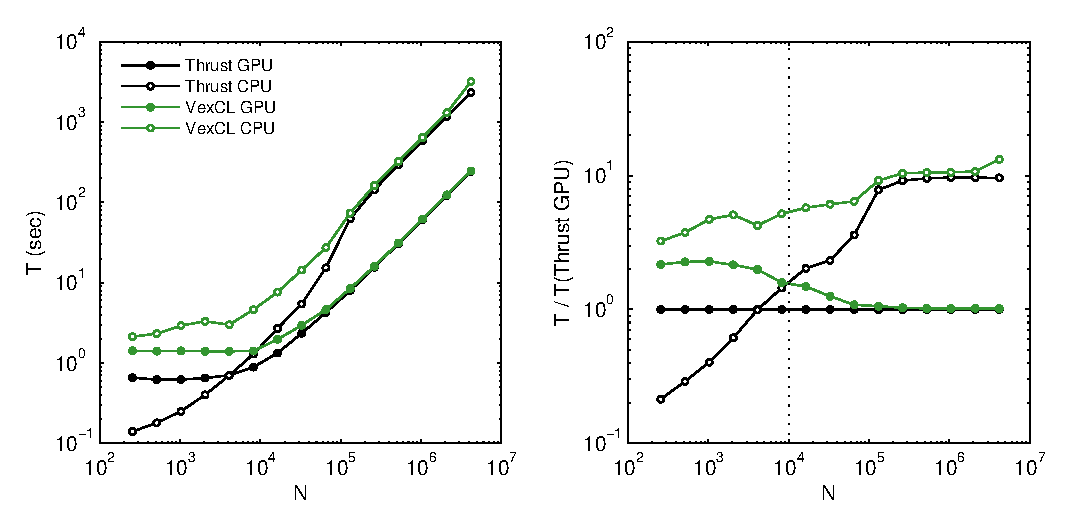
\includegraphics[width=\textwidth]{perfcmp}
        \begin{description}
            \item[GPU:] NVIDIA Tesla C2070
            \item[CPU:] Intel Core i7 930
        \end{description}
    \end{figure}
\end{frame}

\note[itemize]{
\item But let's see what performance we managed to achieve.
\item On the left plot you see absolute running times for problems of different
    sizes. odeint supports Thrust as a backend, so black lines correspond to
    Thrust based solution on a CPU and GPU, red lines is our initial variant
    with VexCL, blue line is our custom kernel, and magenta line is our
    generated kernel. Filled markers are CPU solutions, and empty markers are
    GPU solutions.
\item Right plot shows running times relative to a Thrust GPU solution.
\item You see that both CUDA and OpenCL have high overhead for small problems,
    so CPU-based Thrust solution is the fastest there.
\item But results for larger problems are much more interesting. Our simple
    VexCL variant shows performance similar to Thrust's. The solution on a GPU
    is ten times faster than on a CPU. And both our custom and auto-generated
    kernels are ten times faster than Thrust or simple VexCL. And generated
    kernel is even a bit faster than our manual kernel. That's probably
    because all constants are hard-coded in the kernel source.
}

%----------------------------------------------------------------------------
\begin{frame}[fragile]{Multigpu scalability}
    \begin{columns}
        \begin{column}{0.45\textwidth}
            \begin{itemize}
                \item \emph{Larger} problems may be solved\\ on the same system.
                \item Large problems may be solved \emph{faster}.
            \end{itemize}
        \end{column}
        \begin{column}{0.5\textwidth}
            \begin{figure}
                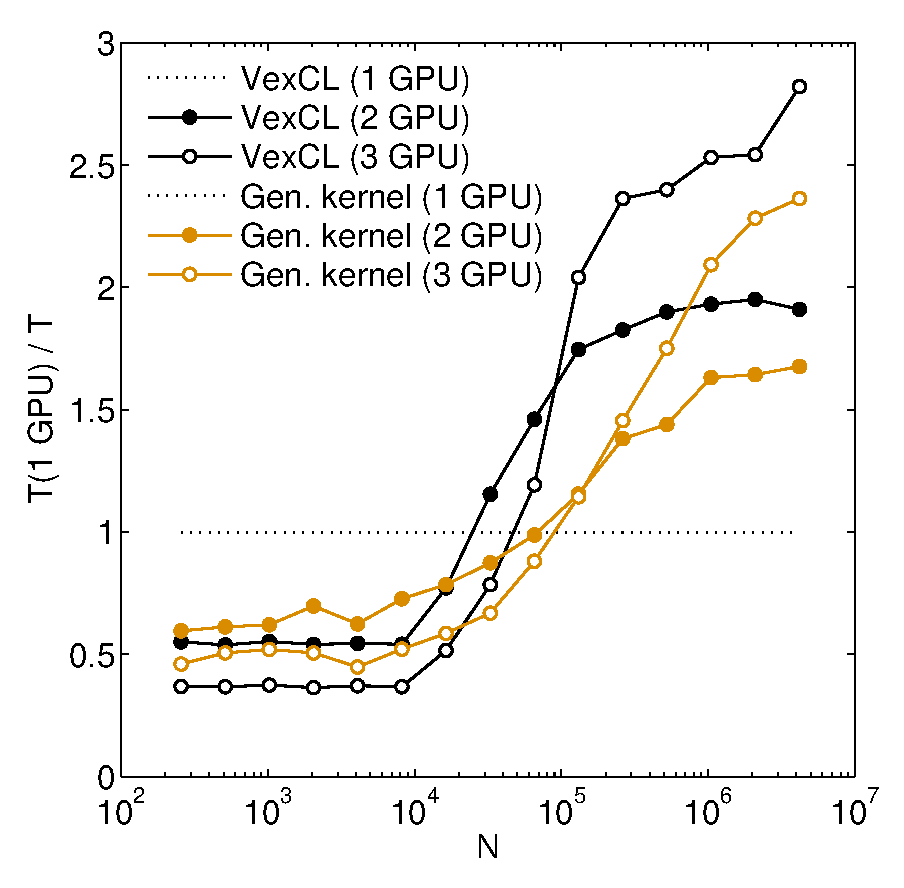
\includegraphics[width=\textwidth]{scaling}
            \end{figure}
        \end{column}
    \end{columns}
\end{frame}

\note[itemize]{
\item While we look at performance, let see how well VexCL scales with use of
    multiple GPUs.
\item Here you see acceleration that we get from using several GPUs for simple
    variant and for generated kernel.
\item Ideally, we would get double acceleration from two cards, and triple
    acceleration from three cards. And we are getting close to these numbers
    for large problem sizes.
\item Another advantage of multigpu approach is that you can solve larger
    problems on the same system, because memory is split between all your
    devices.
}

\section{Implementation details}

%----------------------------------------------------------------------------
\begin{frame}{}
    \tableofcontents[currentsection,hideallsubsections]
\end{frame}

\note{ }

\subsection{Expression trees}

%----------------------------------------------------------------------------
\begin{frame}[fragile]{Expression trees}
    \begin{itemize}
        \item VexCL is an \emph{expression template} library
        \item Each expression in the code results in an expression tree
            evaluated at time of assignment.
            \begin{itemize}
                \item No temporaries are created
                \item Single kernel is generated and executed
            \end{itemize}
    \end{itemize}
    \begin{exampleblock}{Example expression}
        \begin{onlyenv}<1|handout:0>
            \begin{lstlisting}
x = 2 * y - sin(z);
            \end{lstlisting}
        \end{onlyenv}
        \begin{onlyenv}<2>
            \begin{lstlisting}[escapechar=!]
x = !\color{darkred}{2.0}! * y - sin(z);
            \end{lstlisting}
        \end{onlyenv}
    \end{exampleblock}
    \begin{figure}
        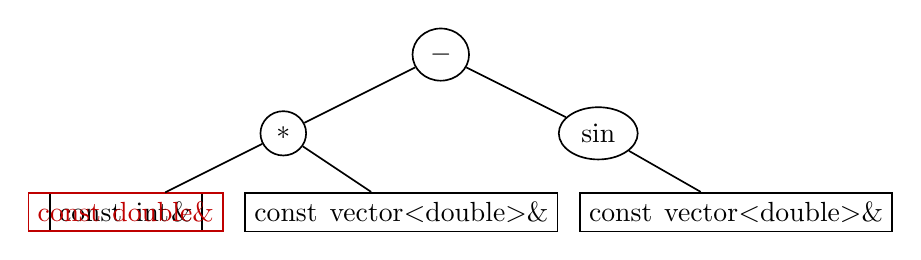
\begin{tikzpicture}
            \draw (0,0) node(minus)[draw,ellipse]{$-$};
            \draw (minus) +(-2, -1) node(times)[draw,ellipse]{$*$};
            \draw (minus) +(2, -1) node(sine)[draw,ellipse]{\code{sin}};
            \uncover<1|handout:0>{
            \draw (times) +(-2,-1) node(const)[draw]{\code{const int&}};
            }
            \uncover<2>{
            \draw (times) +(-2,-1) node(const)[draw,darkred]{\code{const double&}};
            }
            \draw (times) +(1.5,-1) node(v1)[draw]{\code{const vector<double>&}};
            \draw (sine) +(1.75,-1) node(v2)[draw]{\code{const vector<double>&}};

            \draw (minus) -- (times);
            \draw (minus) -- (sine);
            \draw (times) -- (const);
            \draw (times) -- (v1);
            \draw (sine) -- (v2);
        \end{tikzpicture}
    \end{figure}
\end{frame}

\note[itemize]{
\item Kernel for an expression is generated and compiled only first time the
    expression is encountered. Same overhead exists for manually written OpenCL
    applications.
\item The type of an expression tree encodes types of all its subexpressions,
    so for example this expression would result in a different type and
    different kernel.
\item You should keep this in mind if you want to minimize number of generated
    kernels.
}

\subsection{Kernel generation}

%----------------------------------------------------------------------------
\begin{frame}[fragile]{Kernel generation}
    \begin{columns}
        \begin{column}{0.38\textwidth}
            \begin{exampleblock}{The expression}
                \begin{lstlisting}
x = 2 * y - sin(z);
                \end{lstlisting}
            \end{exampleblock}
        \end{column}
        \begin{column}{0.55\textwidth}
            \emph{Define \code{VEXCL_SHOW_KERNELS} to see the generated code.}
        \end{column}
    \end{columns}
    \begin{exampleblock}{\ldots results in this kernel:}
        \begin{lstlisting}
kernel void minus_multiplies_term_term_sin_term(
    ulong n,
    global double *res,
    int prm_1,
    global double *prm_2,
    global double *prm_3
)
{
    for(size_t idx = get_global_id(0); idx < n; idx += get_global_size(0)) {
        res[idx] = ( ( prm_1 * prm_2[idx] ) - sin( prm_3[idx] ) );
    }
}
        \end{lstlisting}
    \end{exampleblock}
\end{frame}

\note[itemize]{
\item To generate a kernel from an expression VexCL needs to create a parameter
    list for the kernel and the expression string in the kernel body.
\item Expression tree terminals become kernel parameters, and the expression
    string is formed from the information encoded in the expression tree.
\item Here is an example of kernel that is generated from this simle
    expression.
\item If you are curious, you can define \code{VEXCL_SHOW_KERNELS} macro
    before vexcl include pragma. Then sources of every generated kernel will be
    flushed to standard output.
}

\subsection{Performance tip}

%----------------------------------------------------------------------------
\begin{frame}[fragile]{Performance tip}
    \begin{itemize}
        \item No way to tell if two terminals refer to the same data!
        \item Example: finding number of points in 1st quadrant
    \end{itemize}
    \begin{exampleblock}{Naive}
        \begin{lstlisting}
return sum( 0.0 <= atan2(y, x) && atan2(y, x) <= M_PI/2 );
        \end{lstlisting}
    \end{exampleblock}
    \begin{itemize}
        \item<alert@1> \code{x} and \code{y} are read twice
        \item<alert@1> \code{atan2} is computed twice
    \end{itemize}
    \begin{exampleblock}{Using custom function}
        \begin{lstlisting}
return sum( between(0.0, atan2(y, x), M_PI/2) );
        \end{lstlisting}
    \end{exampleblock}
\end{frame}

\note[itemize]{
\item Another advice: with current implementation there is no way for VexCL to
    tell if two terminals are actually the same vector object.
\item So you can use custom function to minimize global memory reads and reduce
    number of operations.
}

\subsection{Custom kernels}

%----------------------------------------------------------------------------
\begin{frame}[fragile]{Custom kernels}
    \begin{exampleblock}{It is possible to use custom kernels with VexCL vectors}
        \begin{lstlisting}
vex::vector<float> x(ctx.queue(), n);

for(uint d = 0; d < ctx.size(); d++) {
    cl::Program program = build_sources(ctx.context(d),
        "kernel void dummy(ulong size, global float *x) {\n"
        "    x[get_global_id(0)] = 4.2;\n"
        "}\n");

    cl::Kernel dummy(program, "dummy");

    dummy.setArg(0, static_cast<cl_ulong>(x.part_size(d)));
    dummy.setArg(1, x(d));

    ctx.queue(d).enqueueNDRangeKernel(dummy, cl::NullRange, x.part_size(d), cl::NullRange);
}
        \end{lstlisting}
    \end{exampleblock}
\end{frame}

\note[itemize]{
\item You can also create custom kernels, but you have to remember that vectors
    are split between compute devices.
\item You have to compile the kernel for each of the devices in context.
\item vector member functions \code{part_start()} and \code{part_size()}
    provide the position of a local device part in a vector and the size of
    vector part that is stored on a device.
\item vector braces operator returns local OpenCL buffer that holds partial
    data.
}

\section{Conclusion}

%----------------------------------------------------------------------------
\begin{frame}{Conclusion and Questions}
    \begin{itemize}
        \item VexCL allows to write compact and readable code\\
            without sacrificing too much performance.
        \item Multiple compute devices are employed transparently.
        \item Supported compilers (don't forget to enable C++11 features):
            \begin{itemize}
                \item GCC v4.6
                \item Clang v3.1
                \item MS Visual C++ 2010 (partially)
            \end{itemize}
    \end{itemize}

    \begin{columns}
        \begin{column}{0.5\textwidth}
            \begin{itemize}
                \item \href{https://github.com/ddemidov/vexcl}
                    {https://github.com/ddemidov/vexcl}
            \end{itemize}
        \end{column}
        \begin{column}{0.25\textwidth}
            \begin{figure}
                \includegraphics[width=0.9\textwidth]{oktobercat}
            \end{figure}
        \end{column}
        \begin{column}{0.1\textwidth}
        \end{column}
    \end{columns}
\end{frame}

\note{ }

\appendix

\section{Conjugate gradients method}

\begin{frame}[fragile,shrink=20]{Conjugate gradients method}
    \begin{exampleblock}{Solve linear equations system $Au = f$}
        \begin{lstlisting}
void cg::solve(const vex::SpMat<double> &A, const vex::vector<double> &f, vex::vector<double> &u) {
    // Member fields:
    // vex::vector<double> r, p, q;
    // Reductor<double,MAX> max; Reductor<double,SUM> sum;

    double rho1 = 0, rho2 = 1;
    r = f - A * u;

    for(int iter = 0; max( fabs(r) ) > 1e-8 && iter < n; iter++) {
        rho1 = sum(r * r);

        if (iter == 0) {
            p = r;
        } else {
            double beta = rho1 / rho2;
            p = r + beta * p;
        }

        q = A * p;

        double alpha = rho1 / sum(p * q);

        u += alpha * p;
        r -= alpha * q;

        rho2 = rho1;
    }
}
        \end{lstlisting}
    \end{exampleblock}
\end{frame}

\note {}

\section{Generated kernel}

%----------------------------------------------------------------------------
\begin{frame}[fragile,shrink=50]{The generated kernel (is ugly)}
    \begin{exampleblock}{}
        \begin{lstlisting}
kernel void lorenz(
	ulong n,
	global double* p_var0,
	global double* p_var1,
	global double* p_var2,
	global const double* p_var3
	)
{
size_t idx = get_global_id(0);
if (idx < n) {
double var0 = p_var0[idx];
double var1 = p_var1[idx];
double var2 = p_var2[idx];
double var3 = p_var3[idx];
double var4;
double var5;
double var6;
double var7;
double var8;
double var9;
double var10;
double var11;
double var12;
double var13;
double var14;
double var15;
double var16;
double var17;
double var18;
var4 = (1.000000000000e+01 * (var1 - var0));
var5 = (((var3 * var0) - var1) - (var0 * var2));
var6 = ((var0 * var1) - (2.666666666666e+00 * var2));
var7 = ((1.000000000000e+00 * var0) + (5.000000000000e-03 * var4));
var8 = ((1.000000000000e+00 * var1) + (5.000000000000e-03 * var5));
var9 = ((1.000000000000e+00 * var2) + (5.000000000000e-03 * var6));
var10 = (1.000000000000e+01 * (var8 - var7));
var11 = (((var3 * var7) - var8) - (var7 * var9));
var12 = ((var7 * var8) - (2.666666666666e+00 * var9));
var7 = (((1.000000000000e+00 * var0) + (0.000000000000e+00 * var4)) + (5.000000000000e-03 * var10));
var8 = (((1.000000000000e+00 * var1) + (0.000000000000e+00 * var5)) + (5.000000000000e-03 * var11));
var9 = (((1.000000000000e+00 * var2) + (0.000000000000e+00 * var6)) + (5.000000000000e-03 * var12));
var13 = (1.000000000000e+01 * (var8 - var7));
var14 = (((var3 * var7) - var8) - (var7 * var9));
var15 = ((var7 * var8) - (2.666666666666e+00 * var9));
var7 = ((((1.000000000000e+00 * var0) + (0.000000000000e+00 * var4)) + (0.000000000000e+00 * var10)) + (1.000000000000e-02 * var13));
var8 = ((((1.000000000000e+00 * var1) + (0.000000000000e+00 * var5)) + (0.000000000000e+00 * var11)) + (1.000000000000e-02 * var14));
var9 = ((((1.000000000000e+00 * var2) + (0.000000000000e+00 * var6)) + (0.000000000000e+00 * var12)) + (1.000000000000e-02 * var15));
var16 = (1.000000000000e+01 * (var8 - var7));
var17 = (((var3 * var7) - var8) - (var7 * var9));
var18 = ((var7 * var8) - (2.666666666666e+00 * var9));
var0 = (((((1.000000000000e+00 * var0) + (1.666666666666e-03 * var4)) + (3.333333333333e-03 * var10)) + (3.333333333333e-03 * var13)) + (1.666666666666e-03 * var16));
var1 = (((((1.000000000000e+00 * var1) + (1.666666666666e-03 * var5)) + (3.333333333333e-03 * var11)) + (3.333333333333e-03 * var14)) + (1.666666666666e-03 * var17));
var2 = (((((1.000000000000e+00 * var2) + (1.666666666666e-03 * var6)) + (3.333333333333e-03 * var12)) + (3.333333333333e-03 * var15)) + (1.666666666666e-03 * var18));
p_var0[idx] = var0;
p_var1[idx] = var1;
p_var2[idx] = var2;
}
}
        \end{lstlisting}
    \end{exampleblock}
\end{frame}

\note{ }

\end{document}


% vim: et
